\documentclass{standalone}
\usepackage{color}
\usepackage{tikz}
\usetikzlibrary{shapes,arrows,arrows.meta,fit,positioning}

\newcommand{\defaultwidth}{6cm}
\tikzset{
    auto, node distance = 2cm,
    stage/.style = { draw, thick, rectangle, align=center,
        text width = \defaultwidth, 
        font=\bfseries,
        rounded corners=2mm, 
        minimum width = \defaultwidth
    },
    note/.style = { draw, very thin, rectangle, dashed, align=center,
        node distance = 0.5cm,
        text width = \defaultwidth - 1cm, 
        font=\footnotesize,
        minimum width = \defaultwidth - 1cm
    },
    arrow/.style = { ->, very thick },
    arrow_text/.style = { align=center,
        pos = 0.5,
        text width = 3cm, 
        font = \scriptsize
    }
}

\begin{document}
    \begin{tikzpicture}
        \node[stage] (0) at (0,0)
            {Points in partition \\ 
            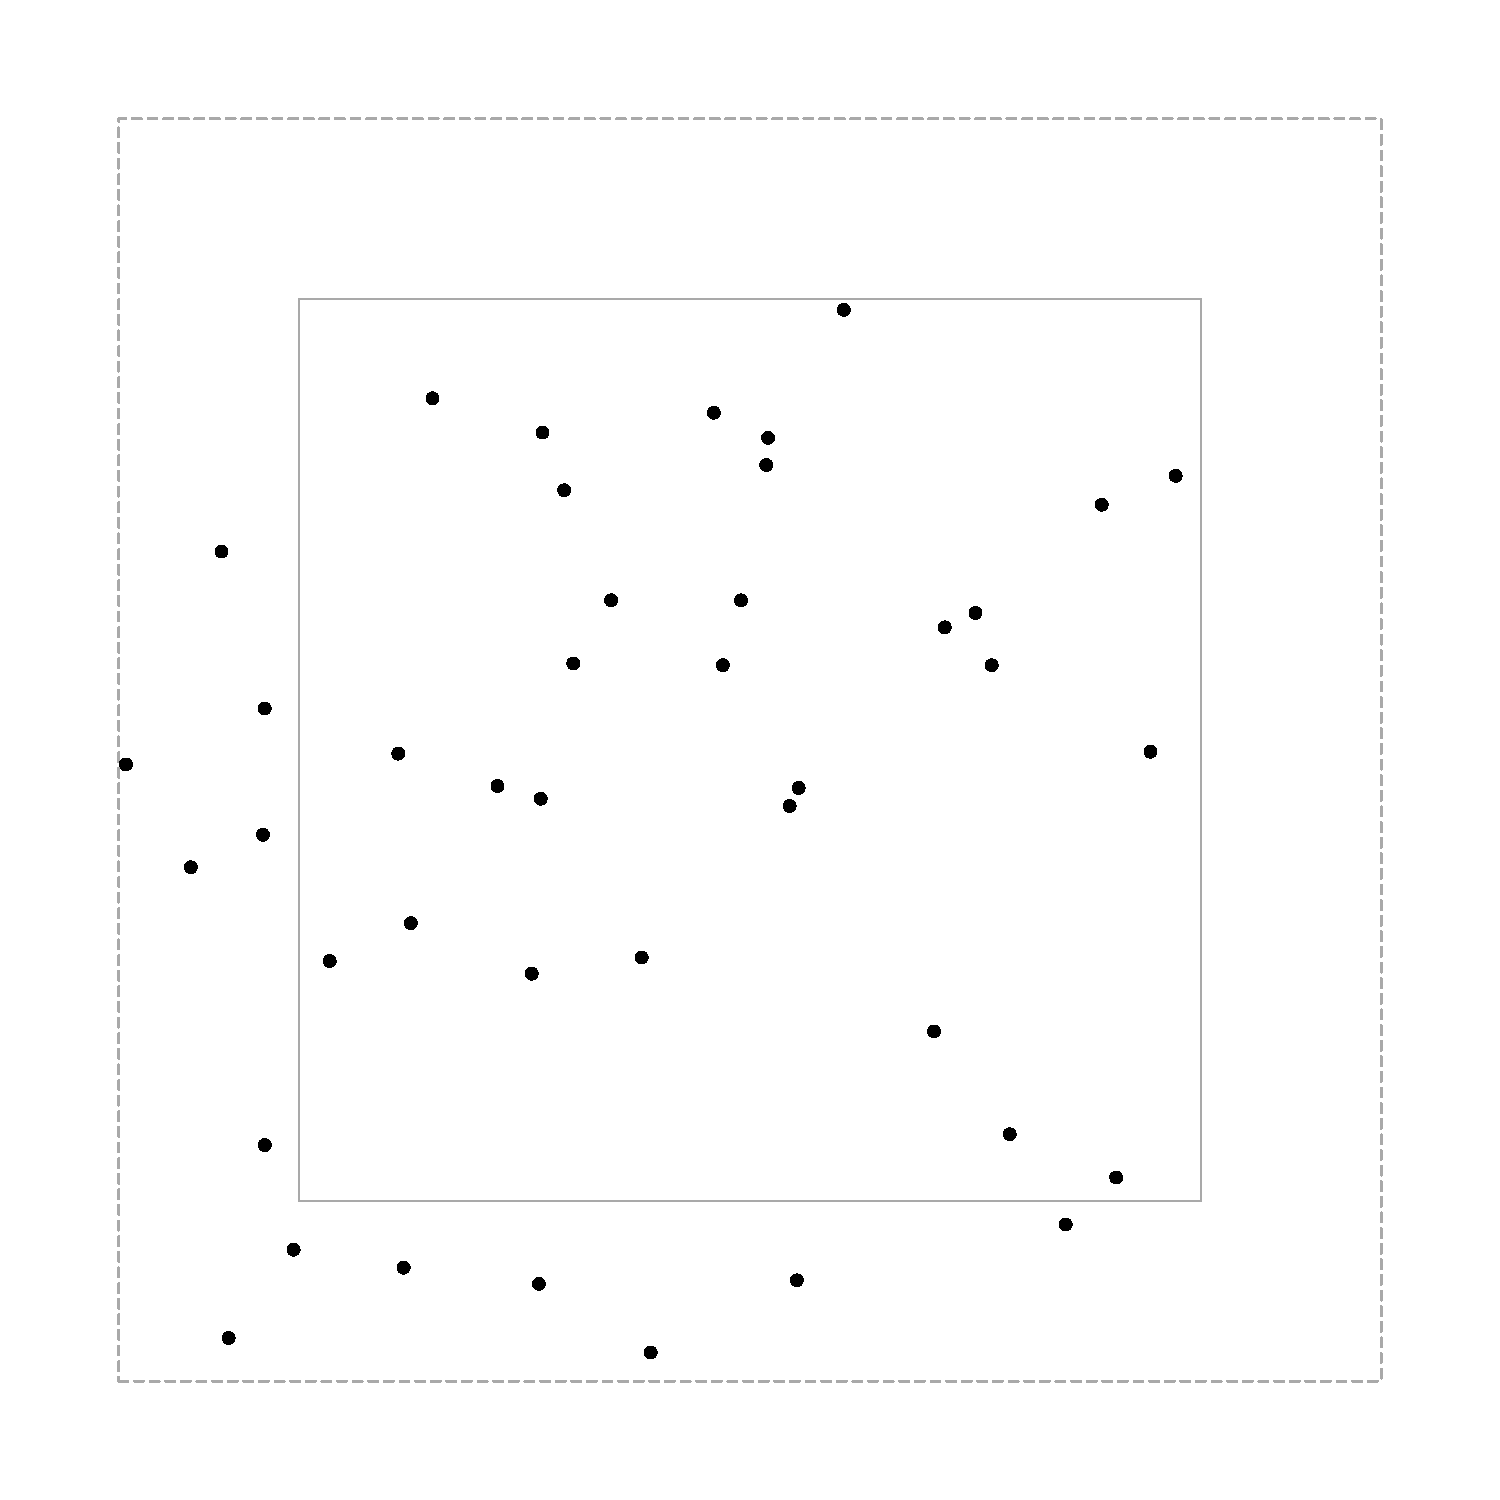
\includegraphics[width=\defaultwidth, page=1]{pflock}};
        \node[stage] (1) [right = of 0]
            {Finding pairs \\ 
            \includegraphics[width=\defaultwidth, page=2]{pflock}};
        \node[stage] (2) [right = of 1] 
            {Computing centers \\ 
            \includegraphics[width=\defaultwidth, page=3]{pflock}};
        \node[stage] (3) [right = of 2] 
            {Finding disks \\ 
            \includegraphics[width=\defaultwidth, page=4]{pflock}};
        \node[stage] (4) [right = of 3] 
            {Pruning disks \\ 
            \includegraphics[width=\defaultwidth, page=5]{pflock}};
                        
        \draw[arrow] (0) -- node[arrow_text]{Points}    (1);
        \draw[arrow] (1) -- node[arrow_text]{Pairs}      (2);
        \draw[arrow] (2) -- node[arrow_text]{Centers} (3);
        \draw[arrow] (3) -- node[arrow_text]{Disks}     (4);
        
    \end{tikzpicture}
\end{document}
